% Complete project explanation — written to be the source material for slides and for the dissertation.
\documentclass[11pt,a4paper]{article}
\usepackage[margin=2.3cm]{geometry}
\usepackage{graphicx}\usepackage{booktabs}\usepackage{xcolor}\usepackage{titlesec}
\usepackage{enumitem}\usepackage[hidelinks]{hyperref}\usepackage{helvet}\usepackage{parskip}
\usepackage{tcolorbox}\usepackage{longtable}
\renewcommand{\familydefault}{\sfdefault}

\definecolor{ink}{HTML}{1D2227}\definecolor{blue}{HTML}{31708F}\definecolor{gold}{HTML}{B07D2B}
\definecolor{soft}{HTML}{5A636C}\definecolor{green}{HTML}{3C7A4E}\definecolor{red}{HTML}{9E3B33}
\definecolor{wash}{HTML}{EEF3F6}

\titleformat{\section}{\Large\bfseries\color{ink}}{\thesection}{0.7em}{}
\titleformat{\subsection}{\large\bfseries\color{blue}}{\thesubsection}{0.6em}{}
\setlist{nosep,leftmargin=1.3em}
\newtcolorbox{key}[1][]{colback=wash,colframe=blue,boxrule=0.6pt,left=8pt,right=8pt,top=6pt,bottom=6pt,#1}
\newcommand{\say}[1]{\textit{\color{soft}#1}}

\begin{document}

\begin{center}
{\Huge\bfseries Visualising Emotion}\\[8pt]
{\Large Does an AI drawing carry the feeling in the words that made it?}\\[14pt]
{\color{soft}\large A complete explanation of the project}\\[10pt]
{\color{soft}MSc Artificial Intelligence dissertation · Shre Hari Prem Anandh}\\
{\color{soft}Supervisor: Dr Chaona Chen · University of Sheffield}\\[4pt]
{\color{soft}\small Every figure in this document was verified against the analysis on 1 September 2026}
\end{center}
\vspace{6pt}\hrule\vspace{12pt}

\begin{key}
\textbf{The project in one paragraph.} At the Festival of the Mind 2024, about a thousand members of
the public typed a few words about how they were feeling, and DALL$\cdot$E drew each entry as a
black-and-white line drawing. This project builds and validates a way to measure whether the drawing
carries the feeling that was in the words. It finds that alignment is real and well above chance,
that it is much stronger when the drawing contains a readable face than when it is a scene, that the
generator is inconsistent with itself, and that the method used to measure it matters a great deal.
\end{key}

\section{The question}

You can already check whether an AI drew what a prompt asked for, provided the prompt names objects.
Ask for \say{a red car} and a metric can look for a car and check that it is red. That is what most
text-to-image evaluation does.

Feelings do not work that way. If somebody types \say{tired but happy}, there is no object to look
for. There is no agreed answer key. And the feeling is mixed, which most emotion tools handle badly.

\begin{key}
\textbf{The precise question this project answers:}\\[4pt]
To what extent does an automatic image-emotion reader agree with prompt-derived emotion labels for
AI-generated monochrome drawings, and how does that agreement vary by visual content and by repeated
prompts?
\end{key}

That wording matters, and it is deliberately narrower than \say{does the drawing convey the
feeling}. This project measures \textbf{agreement between two automatic systems} — one reading the
words, one reading the drawing. It does not establish that a human viewer perceives the same
feeling. That distinction is carried honestly through everything that follows.

\section{Why the question is open}

97 papers were collected, read and triaged; 73 were kept as core evidence and organised into twelve
themes. The literature establishes four things that, taken together, leave a gap.

\begin{itemize}
\item \textbf{Emotion in text is well studied.} GoEmotions supplies a 27-category taxonomy, a large
labelled corpus and an off-the-shelf classifier. But short, first-person self-report is the hardest
register for these tools, and free self-report resolves roughly 27 blended categories rather than a
tidy handful.
\item \textbf{Emotional image \emph{generation} is well studied.} Systems exist that deliberately
make images carry a chosen emotion. Notably, the strongest evidence says lightness and chroma —
not hue, and not shape — carry most of the emotional meaning in text-to-image output.
\item \textbf{Text-to-image \emph{evaluation} is well studied, but for objects.} The metrics score
whether the picture contains what the prompt named. Recent work shows these metrics are fragile
enough to be flipped by small perturbations.
\item \textbf{Reading emotion back out of an image is possible but weak.} Vision-language models are
positively biased and order-sensitive readers of emotion.
\end{itemize}

\begin{key}
\textbf{The gap.} Nobody has checked whether the feeling in a person's own unedited words survives
the journey into a drawing. This dataset is unusually well suited to asking: the prompts are real,
first-person, short and often mixed; and because the drawings are monochrome line art, the channel
the literature says usually carries emotion — colour — is simply absent.
\end{key}

\textbf{An important restraint.} The colour literature motivates why this dataset is a hard case. It
is \emph{not} a result of this project. There is no colour-control condition here, so no claim is
made about the effect of removing colour. Every finding applies within this monochrome corpus.

\section{The dataset, and what it took to use it}

\begin{center}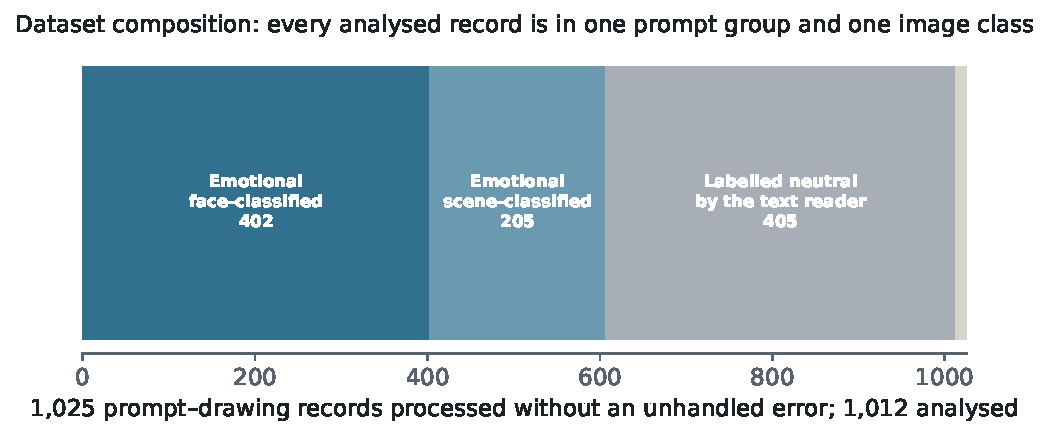
\includegraphics[width=0.95\textwidth]{../figures/fig5_dataset.pdf}\end{center}

1,025 text--image pairs. Median prompt length is about four words. Before any analysis, three
properties had to be handled.

\begin{itemize}
\item \textbf{Three incompatible filename schemes} in one folder: \texttt{img\_00001.PNG} for ids
1--199, \texttt{img\_200.PNG} for 200--999, \texttt{img\_t1000.PNG} for 1000 and above --- and two
files use a lowercase extension. A naive loader resolves under 20\% of the corpus; the loader written
here resolves 100\%.
\item \textbf{Hidden provenance metadata.} Every PNG carries a C2PA/JUMBF manifest containing an
RFC-3161 signing timestamp. Recovering it gave a creation time per image and revealed that
\textbf{records 1--13 were generated before the festival} --- developer tests. They are processed but
excluded from analysis, so nothing is silently dropped.
\item \textbf{Repeated prompts.} 87 distinct prompts were drawn more than once, covering 336 records.
This looked like a nuisance and became a finding.
\end{itemize}

\begin{center}
\begin{tabular}{@{}lr@{}}
\toprule
\textbf{Dataset accounting} & \textbf{Records}\\
\midrule
Processed by the pipeline (0 failures) & 1{,}025\\
Pre-festival developer tests, excluded & 13\\
\textbf{Analysed} & \textbf{1{,}012}\\
\quad of which the words carry a feeling & 607\\
\quad of which the words carry no feeling (the control) & 405\\
\quad drawings with a readable face & 591\\
\quad drawings with no readable face (scenes) & 421\\
Distinct prompts (identity from pre-redaction text) & 763\\
Records repeating an earlier prompt & 249\\
\bottomrule
\end{tabular}
\end{center}

\section{The method}

The supervisor's instruction was decisive: \textbf{never ask a vision model what emotion a picture
shows.} Describe the picture in plain factual terms, then infer the feeling from that description
with a separate model. The pipeline implements exactly that.

\subsection{Stage by stage}

\begin{enumerate}
\item \textbf{Load and redact.} Prompts are loaded through a single loader that applies name
redaction, so the analysis, the figures and the demo app cannot diverge.
\item \textbf{Describe.} BLIP-VQA is asked five fixed questions about the drawing: \say{What is the
facial expression?}, \say{What is the person doing?}, \say{What is the body posture?}, \say{How many
people are there?}, \say{What is in the picture?} The answers are assembled into one neutral
sentence. \textbf{The word ``emotion'' never appears in any question.}
\item \textbf{Extract, image side.} A zero-shot natural-language-inference model reads that
description against the hypothesis template \say{This scene conveys \{\}.} across seven emotion
families, returning a ranked distribution.
\item \textbf{Extract, text side.} GoEmotions reads the person's own words, and its 27 categories are
collapsed onto the same seven families, so both sides live in one label space.
\item \textbf{Compare.} Four similarity measures, each referenced to chance.
\end{enumerate}

\subsection{Models used}

\begin{center}
\begin{tabular}{@{}llp{5.6cm}@{}}
\toprule
\textbf{Model} & \textbf{Size} & \textbf{Role}\\
\midrule
\texttt{Salesforce/blip-vqa-base} & $\sim$385M & Describes the drawing (five questions)\\
\texttt{facebook/bart-large-mnli} & $\sim$407M & Reads a feeling from that description\\
\texttt{SamLowe/roberta-base-go\_emotions} & $\sim$125M & Reads a feeling from the person's words\\
\midrule
OpenCLIP ViT-B/32 (LAION-2B) & $\sim$151M & \emph{Frozen baseline only} --- the older
``ask CLIP directly'' method, kept for comparison\\
\bottomrule
\end{tabular}
\end{center}

\subsection{The four similarity measures}

Similarity, not matching --- \say{happy} and \say{excited} should count as close, not as a miss.

\begin{enumerate}
\item \textbf{Valence--arousal similarity.} Each side's ranked emotions are collapsed to a single
point on a pleasantness/energy plane using fixed centroid coordinates per emotion, and the measure is
one minus the normalised distance between the two points. \emph{This is a designed proxy built on
hand-set centroids, not a continuous lexicon rating.}
\item \textbf{Valence-sign agreement.} Do both sides land on the same side of pleasant/unpleasant?
\item \textbf{Emotion-family agreement.} Do both sides pick the same emotion family outright?
\item \textbf{Top-3 overlap.} How much of the two ranked distributions actually coincides?
\end{enumerate}

\section{What was tried and rejected}

Each link was tested before being trusted. The failures shaped the design and are findings in their
own right.

\begin{center}
\begin{tabular}{@{}p{4.9cm}p{9.3cm}@{}}
\toprule
\textbf{Approach} & \textbf{Why it was rejected (evidence)}\\
\midrule
GoEmotions on the image descriptions & Collapses to \emph{neutral} above 0.95. It is trained on
first-person feeling words; a third-person visual description contains none.\\
A single BLIP caption fed to the reader & Captions too terse (\say{a man with hands in the air});
the reader collapses to \emph{surprise} for almost everything.\\
BART-MNLI on the \emph{prompt} side & Over-reads \emph{surprise} on short first-person text: 333 of
1{,}025 prompts came back as surprise. GoEmotions used instead.\\
Qwen2.5-VL-3B as the describer & 7\,GB in half precision exceeded a 16\,GB laptop; thrashed into
swap with \textbf{zero progress after 4.5 hours}. Never produced a description.\\
Florence-2 as the describer & Hard library incompatibility (\texttt{forced\_bos\_token\_id}) on
transformers 5.14.\\
Asking CLIP directly for the emotion & Beaten head-to-head (see Findings), and manual inspection
found clear errors: arms-raised celebration read as \emph{anger} 0.73.\\
\midrule
\textbf{BLIP-VQA (chosen)} & $\sim$0.4B, roughly 1.5\,s per record, and its ``facial expression''
answer supplies exactly the affective cue the next stage needs.\\
\bottomrule
\end{tabular}
\end{center}

\section{How the numbers are kept honest}

This is the part that makes the findings usable, and it is where most of the methodological effort
went.

\subsection{A random-pairing null for every metric}

Within each subset, the image side is shuffled and re-paired against the untouched prompt side, and
all four metrics are recomputed. This is repeated \textbf{300 times} with a fixed seed. The average
is the chance level; the spread gives a $z$-score. Every number reported in this project is quoted
against its own null. A result counts only insofar as it beats chance.

\subsection{A negative control that passes}

\begin{center}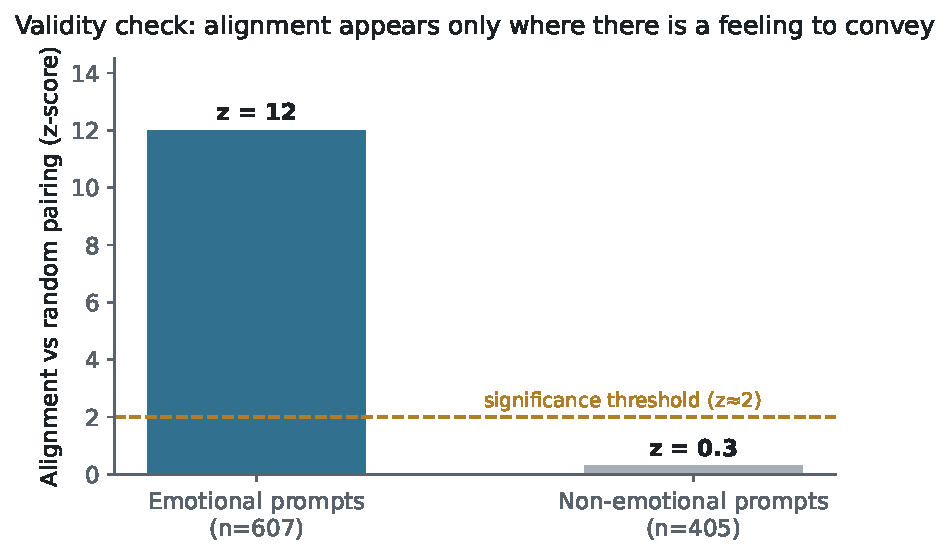
\includegraphics[width=0.78\textwidth]{../figures/fig3_validity_check.pdf}\end{center}

405 of the 1{,}012 prompts contain no feeling at all --- \say{pigs}, \say{mickey mouse},
\say{disney characters}. If the method were finding emotion that was not there, it would score above
chance on these. It does not: valence--arousal similarity is 76.6\% against a null of 76.6\%,
$z=+0.3$; emotion-family agreement sits exactly on its null.

\begin{key}
\textbf{Why this matters more than any single result.} A measurement instrument that reports a signal
where there is none cannot be trusted anywhere. This control is the reason the other numbers can be
believed.
\end{key}

\subsection{A robustness check on repeated prompts}

249 records repeat an earlier prompt, so treating all 1{,}012 as independent would overstate
confidence. Every headline was re-run on the 763 distinct prompts only. All survive, at $z$ between
$+9$ and $+11$.

\subsection{Degenerate nulls are refused}

Where a subset shares one label by construction --- for example the non-emotional records, which are
all neutral --- shuffling cannot change the score, so the ``null'' is an identity rather than a
baseline. These are detected automatically and no chance figure is reported for them.

\section{Chance is not zero}

A late and important discovery, which changed how results are reported.

\begin{key}
The valence--arousal similarity measure \textbf{cannot fall below 41\%} --- that is its mathematical
floor, given the fixed emotion coordinates. Two \emph{randomly paired} records already score about
\textbf{76--77\%}, because most emotions sit close together on the plane.\\[6pt]
So a score of 71\% looks like a pass and is in fact \textbf{below chance}. On a bare 0--100 scale
that is invisible.
\end{key}

There is a second consequence. That measure returns roughly 84\% for face drawings and 83\% for
scene drawings --- it cannot tell them apart. The face/scene difference lives in valence-sign and
emotion-family agreement. The reporting was changed accordingly: those two measures lead, and the
valence--arousal score is always shown against its measured chance line.

\section{Findings}

\subsection{Alignment is real, and much stronger for drawings containing a face}

\begin{center}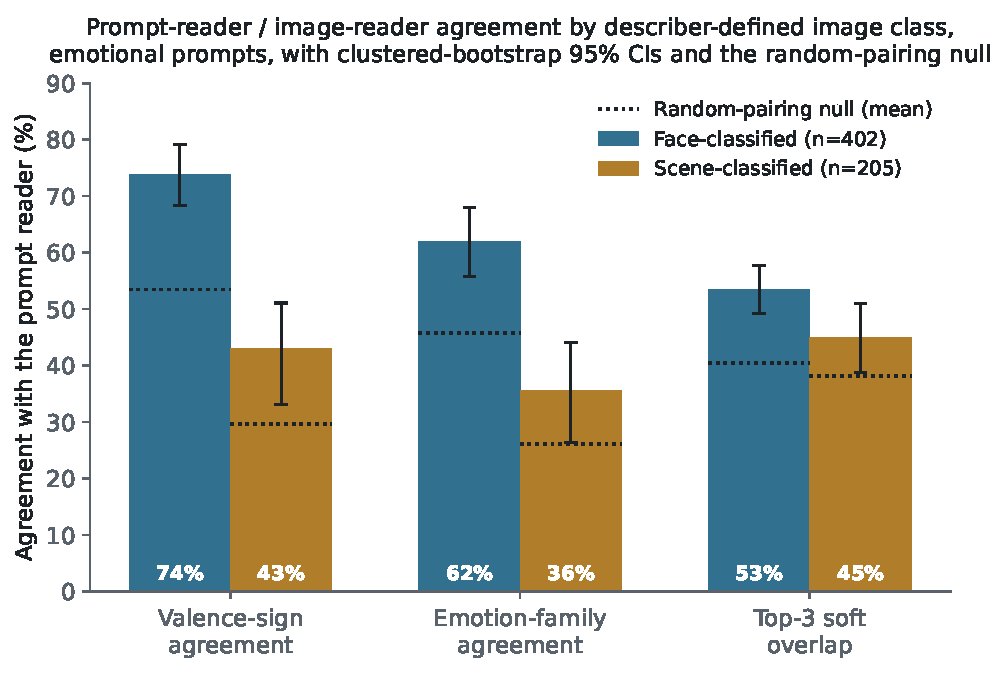
\includegraphics[width=0.9\textwidth]{../figures/fig1_face_vs_scene.pdf}\end{center}

\begin{center}
\begin{tabular}{@{}lccc@{}}
\toprule
\textbf{Emotional prompts only} & \textbf{Valence sign} & \textbf{Emotion family} & \textbf{Top-3 overlap}\\
\midrule
Face drawings ($n=402$)  & \textbf{73.9\%} ($z{+}10.4$) & \textbf{61.9\%} ($z{+}10.3$) & 53.4\% ($z{+}11.6$)\\
Scene drawings ($n=205$) & 42.9\% ($z{+}5.8$) & 35.6\% ($z{+}4.4$) & 44.9\% ($z{+}4.9$)\\
\midrule
All emotional ($n=607$)  & 64.0\% ($z{+}11.1$) & 53.1\% ($z{+}10.3$) & 50.6\% ($z{+}11.6$)\\
\bottomrule
\end{tabular}
\end{center}

Both beat chance. Face drawings align about \textbf{1.7 times better} on both sign and family. On
distinct prompts only, the gap holds: face 71.8\% ($z{+}8.5$) against scene 37.3\% ($z{+}3.5$).

\textbf{Stated carefully:} the pipeline finds stronger prompt--image alignment for drawings it
\emph{classifies} as containing a readable face. It is not evidence that faces inherently carry
emotion, because the classification and the emotion reading share a source --- see Limitations.

\subsection{The generator is inconsistent with itself}

\begin{center}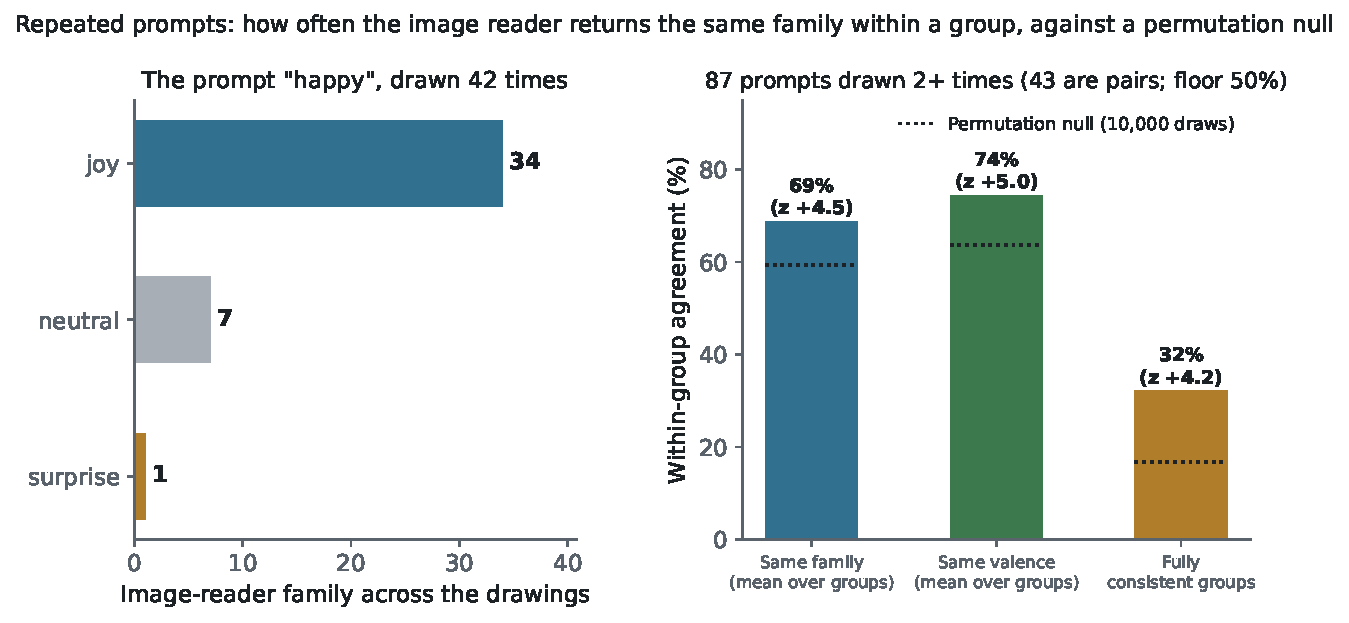
\includegraphics[width=0.92\textwidth]{../figures/fig4_consistency.pdf}\end{center}

87 prompts were drawn between 2 and 42 times each, covering 336 records. Given \emph{identical}
words, the drawings convey the same emotion only \textbf{68.8\%} of the time, and only
\textbf{28 of the 87} repeated prompts are fully consistent across all their drawings. A single
drawing is therefore one sample of the model's behaviour, not a fixed answer --- which is itself a
caution for anyone evaluating generative models on single outputs.

\subsection{The method matters, and the supervisor's architecture wins}

\begin{center}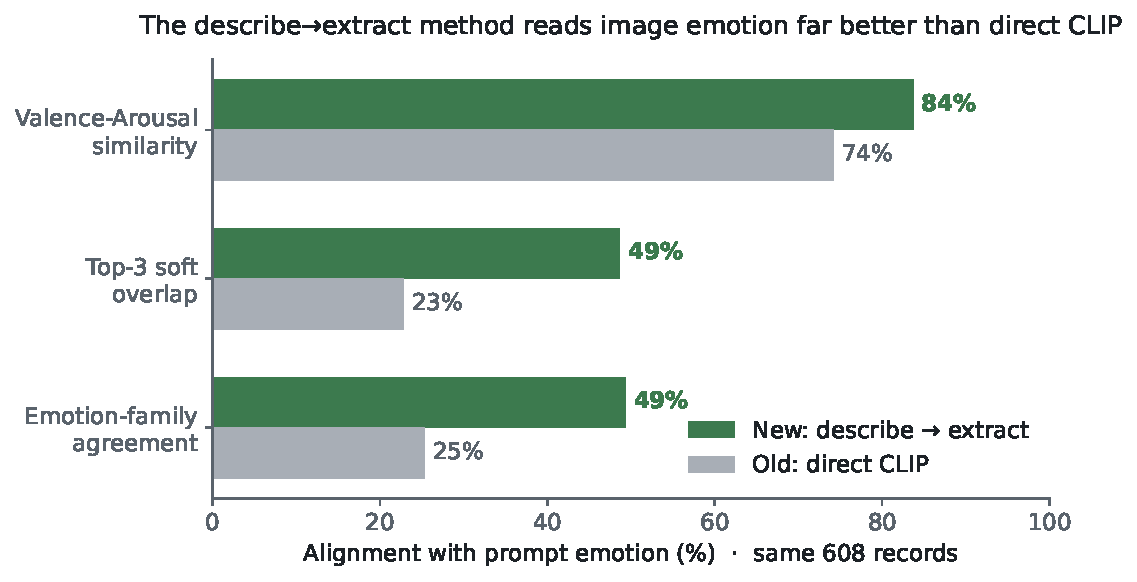
\includegraphics[width=0.88\textwidth]{../figures/fig2_method_comparison.pdf}\end{center}

Head-to-head on the same records, with the prompt side held constant and only the image reader
varied: describe-then-extract reaches \textbf{49.3\%} emotion-family agreement against
\textbf{25.3\%} for asking CLIP directly, and 48.6\% against 22.8\% on top-3 overlap. The redirection
was empirically justified rather than assumed.

\section{The demo application}

A small local web application runs the real pipeline live: choose a drawing from the dataset or
upload an image, see the five factual answers, see both emotion readings side by side, and see the
similarity scored against chance. It exists to make the method inspectable rather than to collect
anything.

Every number it shows is referenced to the measured chance line: the axis starts at the metric's real
floor of 41, the middle half of random pairings is bracketed, and the headline reads \say{closer than
$N$\% of random pairings}. Nothing a visitor types or uploads is stored, and the request log is
suppressed so no visitor IP addresses are recorded.

\section{Ethics and data handling}

No human participants were involved and no new data was collected, so no ethics approval was
required. A human-rating study was designed in full and deliberately \emph{not} run --- approval
alone would have consumed a fortnight of the remaining time. It stands as the clear next study.

\subsection{Name redaction}

Following the supervisor's direction --- redact real names, keep illness and grief content because it
is not identifying on its own and is essential to the analysis, and document the procedure --- a
three-stage pre-processing step was built.

\begin{enumerate}
\item \textbf{Detect}, with deliberately high recall. 77\% of the corpus is written entirely in lower
case, so capitalisation alone would miss most names. Candidates come from a 7{,}944-name gazetteer,
from mid-sentence capitalisation checked against a $\sim$236{,}000-word dictionary, and from naming
phrases such as \say{called X} or \say{my friend X}.
\item \textbf{Review.} Every candidate carries a recorded decision with a reason. Only names of
private individuals are redacted; places, brands, public figures and medical eponyms such as
Parkinson's and Alzheimer's are kept. The audit fails if any candidate is unreviewed.
\item \textbf{Apply}, scoped to the specific record each name was reviewed in.
\end{enumerate}

Eight records contained names of private individuals; those become \texttt{[name]}. Two design
lessons are recorded because both were real errors caught by the audit:

\begin{itemize}
\item \textbf{Unscoped redaction over-reaches.} A bare token list destroyed \say{Jack Frost} and
\say{woolly mammoth}, because those strings occur innocently elsewhere.
\item \textbf{Redaction can forge duplicates.} Two records holding two \emph{different} people's full
names both become \texttt{[name]}, which made the analysis count them as one prompt drawn twice.
Duplicate identity is therefore decided on a key derived from the original text.
\end{itemize}

\textbf{Redaction is analytically inert:} re-running the text-emotion model on the redacted prompts
moves each probability by at most 0.012 and changes \textbf{zero} top-1 emotion families.

Redaction is also a stronger position than withholding records. A hidden set is itself recoverable,
because anyone can probe the public integer ids and read off which are missing. With names redacted,
nothing needs hiding and all 1{,}012 records are shown.

\section{Limitations --- stated plainly}

\begin{enumerate}
\item \textbf{This measures automated agreement, not human perception.} Both readers are models, and
they disagree with each other in opposite directions: the CLIP baseline skews negative on line art,
while the description model reports a happy or smiling expression for 57\% of the faces it can read.
Only human ratings could adjudicate. This is the single most important limitation.
\item \textbf{The face/scene split is partly circular.} It is defined by whether the description
model reported an expression, and the emotion is read from that same description. Scene descriptions
lack expression content, which mechanically lowers their scores. The effect survives the null and
survives deduplication, but it is entangled with its own definition.
\item \textbf{The valence--arousal measure is a designed proxy}, built on hand-set emotion
coordinates. It is not a continuous lexicon-based rating, and it cannot separate faces from scenes.
\item \textbf{No claim is made about colour.} The corpus is monochrome, but there is no colour
condition to compare against.
\item \textbf{No positive-versus-negative direction is claimed.} An earlier claim was withdrawn: the
single-valence subsets have degenerate nulls, and the two readers disagree about the direction.
\item \textbf{Statistical strengthening is still outstanding.} Confidence intervals, a paired test
for the method comparison, and clustered resampling that treats repeated prompts as non-independent
would all strengthen the results chapter.
\end{enumerate}

\section{Reproducibility}

All analysis is driven by scripts with a fixed random seed and no manual steps. An automated test
suite of \textbf{28 checks} covers the environment, data integrity, every analysis, a live run of the
pipeline on fresh images, the redaction procedure and figure regeneration. It currently passes 28/28.
One known weakness is recorded honestly: the figure script contains its numbers literally rather than
reading them from result files, so it cannot detect a change in the analysis on its own.

\section{What this contributes}

\begin{key}
The contribution is \textbf{not} a novel emotion classifier. It is: a question nobody had asked of
real first-person self-report; a dataset that cannot be downloaded; an evaluation design with a
working negative control and null baselines throughout; a demonstrated method comparison; a
repeated-prompt consistency analysis that shows the generator is not deterministic in what it
conveys; and a documented, tested data-protection procedure.
\end{key}

\vspace{6pt}\hrule\vspace{6pt}
{\small\color{soft}All figures and numbers in this document were regenerated and verified against the
analysis on 1 September 2026. Authoritative results file: \texttt{outputs/RESULTS\_final.md}.}

\end{document}
